\chapter{智能结构相变与发育}
\label{chap:intelligence_topological_development}

\begin{chapteroverviewbox}
前面的讨论已经建立了两个彼此耦合但必须区分的结构空间：一方面是认知结构对象构成的
$\mathcal G_C$，另一方面是承载、处理和变换这些认知结构的功能拓扑
$\mathcal G_F$。学习首先表现为 Agent-CSO 在表示、时间尺度、功能位置和内外载体之间的迁移；
当这种迁移长期重复并形成稳定功能关系时，它又可能沉降为新的功能拓扑。
因此，智能发展不能永远被解释为 ``在一个固定结构内部不断增加知识''。
在生命周期足够长、环境足够开放的智能体中，必然出现这样一种情形：
当前功能拓扑仍然能够运行，却已经需要持续支付越来越高的协调代价才能承载新的认知结构流。
此时系统面对的已不再是单纯的状态误差或参数误差，而是
\textbf{认知结构需求与当前功能组织形式之间的结构失配}。

本章由此研究智能动力学中的一个更慢层次：
\begin{statementbox}
\centering
\adjustbox{max width=.96\linewidth}{\(\displaystyle \text{Dynamics on Topology}
\quad\longrightarrow\quad
\text{Dynamics of Topology}\)}
\end{statementbox}
我们将依次建立结构失配、拓扑压力、拓扑重组触发条件、新连接形成、旧连接消退、
功能区域分裂与合并、拓扑捷径、迟滞机制以及最小必要重组原则。
本章尤其强调：
\textbf{拓扑改变不是智能系统面对困难时首先应该采取的策略，而应当是较低成本的状态调整、
表示调整、时间尺度迁移与功能迁移长期无法消除结构残差之后才发生的慢变量改变。}
因此，真正成熟的智能既不能拓扑僵化，也不能结构漂移；
它必须同时维持稳定性与可塑性，并让拓扑变化成为长期经验的结构沉积，而不是瞬时噪声的放大。
\end{chapteroverviewbox}

\begin{figure}[htbp]
\centering
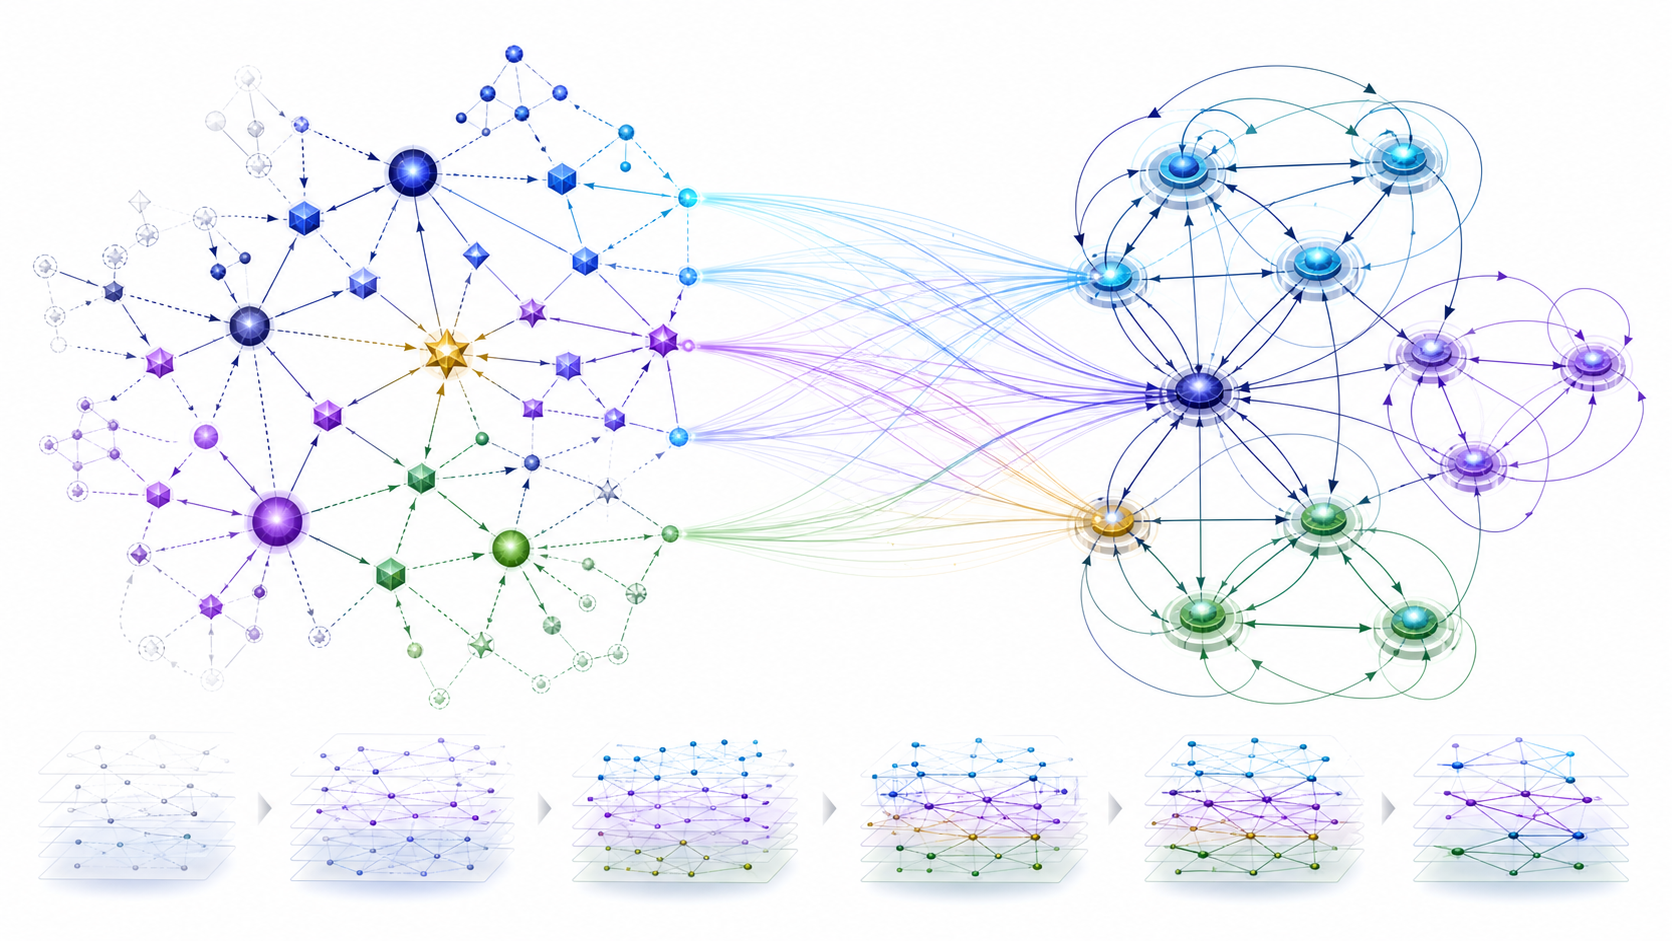
\includegraphics[width=.9\textwidth,height=.38\textheight,keepaspectratio]{images/cognitive-structure-functional-topology.png}
\caption{结构压力、迟滞与最小必要重组}
\end{figure}
\section{结构失配：当认知结构与功能承载不再相称}

在前一章中，我们已经把功能拓扑理解为历史 CSO 流的结构沉积。一个长期稳定的功能连接并不是凭空存在的，
而是某一类 Agent-CSO 在多个功能之间反复迁移、反复完成闭环之后，被系统逐渐固化下来的低成本通路。
因此，任意时刻的功能拓扑 $\mathcal G_F(t)$ 本质上都带有明显的历史性：它更加适合承载系统过去反复遇到的问题，
但并不必然最适合未来将要出现的问题。只要环境、任务集合、身体、工具或智能体自身的认知结构发生持续变化，
当前拓扑就可能逐渐偏离新的结构需求。我们把这种偏离定义为\textbf{结构失配}
（Structural Mismatch）。

为了形式化这一概念，设智能体的功能拓扑为
\[
\mathcal G_F(t)
=
\left(
V_F(t),
E_F(t),
W_F(t)
\right),
\]
认知结构图为
\[
\mathcal G_C(t)
=
\left(
V_C(t),
E_C(t)
\right),
\]
而二者之间存在随时间变化的承载映射
\[
\mu_t:
\mathcal G_C(t)
\rightarrow
\mathcal G_F(t).
\]
这里 $\mu_t$ 并不是一个简单的一对一函数，而更接近多对多的动态关系：
一个 Agent-CSO 可以同时被多个功能协同承载，一个功能也可以在不同上下文中处理大量不同的 Agent-CSO。
我们真正关心的是，在当前 $\mathcal G_F$ 下，某类认知结构是否能够以足够短的路径、足够低的协调成本和足够稳定的闭环被处理。

设 $C_k$ 为某一类持续出现的认知结构，系统为完成它所需要经过的功能路径为
\[
\pi_k
=
(F_{i_1},F_{i_2},\ldots,F_{i_m}),
\]
则可以定义该结构在当前拓扑中的有效承载代价
\[
\mathcal C_{\mathrm{carry}}(C_k|\mathcal G_F)
=
\alpha L(\pi_k)
+
\beta D(\pi_k)
+
\gamma R(\pi_k)
+
\delta U(\pi_k)
+
\eta E(\pi_k),
\]
其中 $L$ 表示路径长度，$D$ 表示跨功能通信延迟，
$R$ 表示为完成任务所需要的重复往返次数，
$U$ 表示不确定性或失配残差，
$E$ 表示额外认知或计算资源消耗。
这里各项并非意味着必须使用这一特定线性形式，而是告诉我们：
所谓结构失配并不是抽象的 ``这个架构看起来不够优雅''，
而应该表现为可观察、可累积的运行代价。

例如，一个智能体长期需要完成同一类任务时，如果每一次任务都必须经过
\[
F_A
\rightarrow
F_B
\rightarrow
F_C
\rightarrow
F_A
\rightarrow
F_D
\rightarrow
F_B
\]
才能闭环，那么问题并不一定意味着这些功能本身不足。
更可能的问题在于：
某种已经变得稳定的认知结构关系仍然被迫通过历史上为其他任务形成的路径进行协调。
如果该任务只出现一次，我们没有理由改变拓扑；
如果这种往返持续数万次，而且每次都表现出相似的 Agent-CSO 流，
那么重复发生的动态过程就开始暴露一个更慢层次的问题：
\begin{statementbox}
当前拓扑没有把长期稳定的功能关系直接表示出来。
\end{statementbox}

因此，我们可以把结构失配写成一类时间平均量：
\[
M_{\mathrm{struct}}(t)
=
\mathbb E_{\Delta T}
\left[
\mathcal C_{\mathrm{carry}}
-
\mathcal C_{\mathrm{expected}}
\right],
\]
其中 $\Delta T$ 必须明显大于普通状态扰动的时间尺度。
这一点非常重要。如果我们直接使用瞬时残差作为结构修改依据，
那么拓扑就会被短期任务、偶然输入和随机噪声不断重写。
成熟智能的结构学习必须区别
\[
\varepsilon_{\mathrm{state}}(t)
\]
与
\[
\overline{\varepsilon}_{\mathrm{struct}}(t).
\]
前者可能只需要一次新的推理、一次注意调整或一次记忆召回；
后者意味着相似的误差在足够长时间内重复出现，并且具有稳定结构。

我们由此得到结构失配的第一个核心判断：

\begin{proposition*}
困难本身不是拓扑改变的证据；
持续以相同结构形式出现的困难才可能是拓扑改变的证据。
\end{proposition*}

这也解释了为什么智能系统不能把 ``没有立即成功'' 与 ``自身架构错误'' 混为一谈。
真正的发育型智能必须能够容忍局部失败，并首先通过已有结构学习。
只有当经验持续表明：
问题并不来自知识不足，而来自知识、功能与闭环之间的组织关系不适配，
系统才应把问题逐渐提升到拓扑层。

从已有科学理论来看，这一思想与自适应网络、结构可塑性、组织学习以及控制系统中的模型失配有相似之处，
但本理论与这些理论之间存在一个重要区别：
我们不是简单研究网络连接是否提高任务性能，而是把\textbf{Agent-CSO 的长期承载轨迹}
作为拓扑变化的主要因果来源。
因此，本章研究的核心不是 ``如何搜索更好的图''，
而是
\begin{statementbox}
一个智能系统如何从自己的生命周期历史中发现：
哪些反复发生的认知过程已经值得成为自身结构的一部分。
\end{statementbox}

\section{拓扑压力：从持续残差到结构重组需求}

结构失配本身并不意味着系统必须立即重构。现实中的智能体始终处在不确定环境中，
任何一次任务都可能产生临时协调成本。如果所有失配都直接转化成拓扑改变，
智能体将处于不断改写自身的状态，最终失去身份连续性、能力稳定性以及可验证的行为边界。
因此，在结构失配与拓扑改变之间，我们需要引入一个中间动力学变量：
\textbf{拓扑压力}（Topological Pressure）。

拓扑压力可以理解为系统内部对 ``当前功能组织方式已经长期不经济'' 的累积证据。
设
\[
P_T(t)
\]
表示拓扑压力，则一个概念性的定义可以写为
\[
P_T
=
F
\left(
\bar{\varepsilon},
\bar{J}_{\mathrm{cross}},
C_{\mathrm{coord}},
L_{\mathrm{latency}},
I_{\mathrm{instability}},
R_{\mathrm{repeat}},
V_{\mathrm{utility}}
\right).
\]
其中 $\bar{\varepsilon}$ 表示长期未消除残差，
$\bar{J}_{\mathrm{cross}}$ 表示长期跨功能的 Agent-CSO 迁移流，
$C_{\mathrm{coord}}$ 表示协调成本，
$L_{\mathrm{latency}}$ 表示路径延迟，
$I_{\mathrm{instability}}$ 表示局部闭环的不稳定程度，
$R_{\mathrm{repeat}}$ 表示同类结构的重复频率，
而 $V_{\mathrm{utility}}$ 则表示如果改善该路径，对整体生命周期能力究竟有多大价值。

为了避免拓扑压力对瞬时噪声过敏，我们可以采用一个慢积分过程：
\[
\tau_T\dot P_T
=
-
P_T
+
\Phi
\left(
\varepsilon,
J^{CSO},
C_{\mathrm{coord}},
L,
U
\right),
\qquad
\tau_T \gg \tau_h.
\]
这意味着拓扑压力具有明显的低通滤波性质。
一次很严重但很偶然的失败未必能够产生持续 $P_T$；
反而是一系列程度并不剧烈、却在数周或数月中不断重复的相同协调模式，
更可能逐渐推动 $P_T$ 上升。

我们可以把这一过程理解为智能系统中的一种慢 ``结构痛感''，
但这里的 ``痛感'' 只是功能隐喻，不涉及主观体验。
它表达的是：
当前系统每一次都能解决问题，
却需要不断支付同一种额外成本。
在短期尺度上，任务仍然成功，因此不存在显著功能崩溃；
在生命周期尺度上，这种重复支付会积累成一个非常明确的结构信号。

设系统对某类任务 $k$ 的实际平均处理成本为
\[
\bar C_k(T),
\]
而其在已有能力条件下可以达到的理论或经验参考成本为
\[
C_k^\star.
\]
则可以定义结构效率比
\[
\eta_k
=
\frac{C_k^\star}{\bar C_k(T)}.
\]
当 $\eta_k\approx 1$ 时，当前拓扑已经能够很好承载该任务；
当 $\eta_k\ll 1$ 且长期保持时，
说明智能体正在重复使用一个明显不经济的功能路径。
但即便如此，拓扑压力仍不能由效率单独决定，
因为一个非常罕见的任务即使代价巨大，也不一定值得修改长期架构。
因此真正影响结构学习的是
\[
R_k \cdot V_k \cdot (1-\eta_k),
\]
也就是重复性、价值和结构低效的共同作用。

进一步说，拓扑压力具有局部性。
并不存在一个全局标量可以完整描述整个 Agent 的结构失配。
更一般的表示是：
\[
P_T(i,j,t),
\]
表示功能区域 $F_i$ 与 $F_j$ 之间产生新耦合、改变现有耦合或重组中间结构的局部压力。
于是整个系统拥有一个拓扑压力场
\[
\mathbf P_T(t)
=
\{P_T(i,j,t)\}.
\]
这使得拓扑学习不必总是 ``重构整个智能体''，
而可以首先表现为局部边权调整、局部功能聚合或局部捷径形成。

本章尤其需要强调：
\[
\boxed{
P_T
\neq
\varepsilon.
}
\]
Residual 告诉系统 ``这次发生了偏差''；
Topological Pressure 告诉系统
``相似偏差已经持续到值得重新审视自己的组织方式''。
前者主要驱动快速认知和局部学习，
后者才有资格进入慢尺度结构治理。

这一区分使整个 AgentOS 的多尺度理论获得了重要连续性。
我们此前已经强调
\[
\boxed{
SlowGovernance\neq FastMicromanagement.
}
\]
现在可以进一步写成：
\begin{statementbox}
\centering
\adjustbox{max width=.96\linewidth}{\(\displaystyle FastError
\nrightarrow
ImmediateTopologyChange.\)}
\end{statementbox}
短期误差首先应被 h、SPC、TCE、CCM、记忆学习和功能迁移吸收。
只有那些无法被这些较快机制长期消化的结构性残差，
才逐渐进入拓扑压力。
这正是一个成熟智能体能够同时保持稳定与发育的基础。

\section{何时当前功能拓扑已经不足}

现在我们面对一个比 ``系统是否犯错'' 更严格的问题：
什么情况下我们可以合理地说，
\textbf{当前功能拓扑本身已经不足以承载智能体正在形成的认知结构}？
如果这一条件不能被清楚定义，拓扑学习就只能退化成随机 Architecture Search；
而如果条件定义得过于苛刻，系统又可能永远停留在早期设计者赋予的固定结构中。

为了解决这一问题，我们首先区分四种不同层级的失败。
第一类是\textbf{状态失败}：
当前状态不正确，但已有结构足以恢复。例如一个规划步骤错误，只需要重新推理。
第二类是\textbf{表示失败}：
当前 CSO 的表示方式不适合问题，需要重新编码、抽象或拆分。
第三类是\textbf{承载失败}：
结构本身是有效的，但当前功能位置、时间尺度或内外载体不合理。
第四类才是\textbf{拓扑失败}：
即使允许充分的状态调整、表示重构和 Agent-CSO 迁移，
系统仍持续需要通过低效路径维持一个稳定而重复的功能关系。

于是我们可以构造一个逐级检验：
\[
\mathcal H_0:
\text{State adjustment is sufficient},
\]
\[
\mathcal H_1:
\text{Representation adaptation is sufficient},
\]
\[
\mathcal H_2:
\text{Timescale/carrier migration is sufficient},
\]
\[
\mathcal H_3:
\text{Functional migration is sufficient},
\]
只有当这些较低层假设长期被数据否定以后，才进入：
\[
\mathcal H_4:
\text{Topology reorganization is necessary}.
\]

换句话说，拓扑不足不是 ``当前架构没有直接支持某个任务''，
而是：
\[
\boxed{
\min_{\text{state,repr.,placement}}
\mathcal L
\left(
\mathcal G_F,
\mu,
C
\right)
>
\theta_{\mathrm{acceptable}},
}
\]
即在保持 $\mathcal G_F$ 不变的条件下，
已经无法通过合理的内部调整把长期损失压缩到可接受区域。

我们可以进一步定义当前拓扑的有效可承载集合：
\[
\mathcal C_{\mathrm{feasible}}
(\mathcal G_F)
=
\left\{
C:
\exists\mu,\,
\mathcal L(C|\mathcal G_F,\mu)
\leq\theta
\right\}.
\]
一个新的 Agent-CSO 并不要求一出现就改变拓扑，
只要它仍然属于
\[
\mathcal C_{\mathrm{feasible}}(\mathcal G_F),
\]
系统就可以通过已有功能组合完成处理。
真正值得发育的是：
越来越多高价值、高频结构长期靠近或超出该可承载边界，
使系统持续工作在高协调、高延迟、高显式认知占用的状态。

这与我们此前关于工作记忆有限性的讨论可以直接连接。
假如某一类已经非常熟悉的任务，每次仍然必须把大量中间关系重新提升到 $h(t)$，
则：
\[
H_{\mathrm{explicit}}(C_k)
\]
长期保持在高水平。
这意味着低层功能没有形成足够稳定的闭环，
导致本应自动化的结构不断占用有限全局认知空间。
因此可以把 ``长期不必要的显式认知占用'' 视为结构失配的重要观测量：
\[
P_T
\propto
\left\langle
H_{\mathrm{explicit}}(C_k)
\right\rangle_T.
\]

这给我们一个非常现实的判断标准。
一个成熟系统不应该因为会做越来越多事情而让 h 越来越拥挤。
恰恰相反，随着学习：
\[
Capability\uparrow,
\qquad
ExplicitCognitiveBurden/Capability\downarrow.
\]
如果能力不断增长，但所有旧能力仍然依赖高层全局推理，
那么系统虽然知识增加，却没有发生真正意义上的认知发育。

因此，在本理论中，
一个功能拓扑 ``不够用'' 的判据不是单一任务性能下降，
而是多个指标在较长时间尺度上共同满足：
高频稳定 CSO 流持续跨越相同功能路径；
协调成本长期不下降；
工作记忆显式占用无法通过技能化进一步减少；
功能间 residual 出现稳定模式；
局部优化已经接近饱和；
新的经验仍不断强化同一种功能依赖。

只有在这些条件共同出现时，
我们才有理由认为：
\begin{statementbox}
当前智能体已经不只是需要学习新的内容，
而是需要学习一种新的组织方式。
\end{statementbox}

\section{新功能连接的形成：从重复迁移到稳定耦合}

拓扑发育最基本的结构事件，是一个原本不存在或非常弱的功能连接逐渐形成。
这一过程不能被理解为系统随意 ``接一条线''，
而应该来自 Agent-CSO 长期迁移历史所提供的统计证据。

设功能节点 $F_i$ 与 $F_j$ 之间的连接权重为
\[
w_{ij}(t).
\]
Agent-CSO 从 $F_i$ 向 $F_j$ 的有效流定义为
\[
J_{ij}^{CSO}(t).
\]
如果某类结构长期反复从 $F_i$ 流向 $F_j$，
我们可以定义其时间平均：
\[
\bar J_{ij}^{CSO}(T)
=
\frac{1}{T}
\int_{t-T}^{t}
J_{ij}^{CSO}(s)\,ds.
\]
但流量本身仍不足以证明连接有价值。
有些高流量只是由于架构缺陷造成的无效往返；
如果直接依据流量强化连接，就可能固化错误。

因此边的生长律必须同时考虑：
\[
Utility_{ij},
\quad
ResidualReduction_{ij},
\quad
LatencySaving_{ij},
\quad
Risk_{ij},
\quad
Cost_{ij}.
\]
一个概念性的连续更新规则可以写成
\[
\tau_T\dot w_{ij}
=
\alpha
\bar J_{ij}^{CSO}
\Delta U_{ij}
+
\beta
\Delta R_{ij}
+
\gamma
\Delta L_{ij}
-
\lambda
C_{ij}
-
\xi
Risk_{ij}.
\]
其中 $\Delta U_{ij}$ 表示该连接对长期效用的改善，
$\Delta R_{ij}$ 表示残差减少，
$\Delta L_{ij}$ 表示延迟降低，
$C_{ij}$ 表示维持该连接所需成本，
而 $Risk_{ij}$ 则约束可能破坏安全边界或权限隔离的结构变化。

如果功能拓扑是离散的，则可以使用更明确的形成条件：
\[
w_{ij}=0
\quad\longrightarrow\quad
w_{ij}>0
\]
当且仅当
\[
\mathbb E_T
\left[
Benefit_{ij}
\right]
-
\lambda Cost_{ij}
-
\xi Risk_{ij}
>
\theta_{\mathrm{on}},
\]
且该条件持续时间达到
\[
T>T_{\min}.
\]

这里的 $T_{\min}$ 极其重要。
它意味着新功能关系必须经过持续经验验证。
换句话说，
AgentOS 的结构发育不能只问：
``建立这条边现在是否有用？''
而应该问：
``在足够多不同情境中，这条关系是否表现出稳定且可泛化的价值？''

例如，假设一个 Agent 最初处理某类视觉事件时，需要：
\[
Perception
\rightarrow
h
\rightarrow
Reasoning
\rightarrow
Action.
\]
经过大量训练以后，系统发现其中某一类视觉模式和某一局部行动之间存在高度稳定关系。
那么该认知结构首先可能经历：
\[
ExplicitCSO
\rightarrow
ExperientialCSO
\rightarrow
GenerativeCSO
\rightarrow
ProceduralCSO.
\]
如果这种下沉仍然依赖多个中间功能节点，
系统就可能进一步形成新的快速耦合，使：
\[
F_{\mathrm{perception}}
\rightarrow
F_{\mathrm{local-control}}
\]
成为更直接的路径。
这时，能力的成熟已经不只是某个参数发生变化，
而是功能图本身对历史经验进行了压缩。

因此可以把边形成解释成：
\begin{statementbox}
过去反复发生的动态关系，
逐渐变成未来不需要重新计算的静态关系。
\end{statementbox}
这就是拓扑作为慢记忆的真正含义。

从计算角度看，一条新功能边类似把反复执行的长路径缓存成快捷调用；
从神经科学类比上看，它与反复共同激活后形成更稳定通路存在某种启发性相似；
从软件工程角度看，它类似把经常跨多个组件协商的路径重新封装成一个稳定服务接口。
但 AgentOS 理论的关键区别在于：
这些结构变化都应该由 Agent-CSO 生命周期流和现实反馈共同驱动，
而不是简单按照共现频率硬编码。

更一般地，新连接形成意味着未来同类 CSO 的传播算子发生了变化。
若原传播为
\[
x(t+\Delta)
=
\mathcal P_{\mathcal G_F}(x(t)),
\]
新增边后变成
\[
x(t+\Delta)
=
\mathcal P_{\mathcal G_F'}(x(t)),
\qquad
\mathcal G_F'\neq\mathcal G_F.
\]
于是，拓扑学习真正改变的是
\textbf{未来认知过程允许怎样传播}，
而不仅是当前知道了什么。

\section{旧连接的消退：遗忘、剪枝与结构释放}

如果拓扑只能增加而不能减少，一个长期智能体最终将形成越来越密集的功能图。
这种系统虽然保留了所有历史路径，却会产生新的问题：
搜索空间扩大、控制耦合增加、异常传播路径增加、功能边界模糊，
最终重新把拓扑复杂度转化成运行时认知负担。
因此真正的发育必须同时包含结构生长与结构消退。

设已有边权为
\[
w_{ij}>0.
\]
如果一条功能关系长期不再承载高价值 CSO 流，
其边权应该允许缓慢衰减。
最简单的形式为
\[
\tau_T\dot w_{ij}
=
-\lambda_d w_{ij}
+
\Phi
\left(
\bar J_{ij}^{CSO},
Utility_{ij},
RecoveryValue_{ij}
\right).
\]
其中 $RecoveryValue_{ij}$ 是非常重要的一项。
一条平时极少使用的安全恢复路径，不能因为使用频率低而被删除；
同样，一些身份、价值和极端异常处理通路可能长期不活跃，
却具有极高潜在重要性。
因此结构删除不能采用单纯的 ``least frequently used'' 原则。

我们可以定义一个边的重要性：
\[
I_{ij}
=
\alpha
Usage_{ij}
+
\beta
Utility_{ij}
+
\gamma
Safety_{ij}
+
\delta
Recovery_{ij}
+
\eta
Identity_{ij}.
\]
只有当
\[
I_{ij}<\theta_{\mathrm{off}}
\]
持续足够长时间，
且其删除不会导致关键闭环断裂时，
才允许：
\[
w_{ij}\rightarrow 0.
\]

这意味着拓扑遗忘必须与普通记忆遗忘区分。
E 中的某个事件可以逐渐失去细节；
某个 Θ 结构可以被更一般模型吸收；
而功能拓扑中的边一旦删除，
改变的是未来整个认知系统的信息传播能力。
因此拓扑遗忘属于更慢、更高风险的结构操作。

我们可以把删除过程划分为三个阶段。
首先是\textbf{边权弱化}：
连接仍存在，但优先级下降。
其次是\textbf{休眠}：
正常路由不再使用，但保留恢复能力。
最后才是\textbf{结构删除}。
因此更合理的状态空间不是
\[
Edge\in\{0,1\},
\]
而是
\[
EdgeState
\in
\{
Active,
Weak,
Dormant,
Retired
\}.
\]
这种多阶段结构能够显著降低灾难性拓扑遗忘。

进一步说，一条边是否应该删除，不能只看局部。
有些边本身使用频率不高，却承担多个闭环之间的桥梁作用。
因此还需要考虑图结构中的介数、可达性和冗余：
\[
Centrality_{ij},
\quad
Reachability,
\quad
Redundancy_{ij}.
\]
如果删除 $e_{ij}$ 会使某个关键 CSO 类失去有效承载路径，
即使其直接使用频率不高，也不应删除。

这对应一个更普遍的智能发育原则：
\begin{proposition*}
成熟不是不断拥有更多结构，
而是保留越来越少但越来越有效的结构。
\end{proposition*}
这和人类技能成熟、软件重构乃至科学理论发展都有某种共同特点：
大量早期显式步骤最终被压缩，
一些冗余中间结构消失，
留下更加稳定、抽象和高效的关系。

不过我们必须避免把这一过程浪漫化。
结构删除可能形成习惯僵化，也可能删除在未来环境重新变得重要的路径。
因此成熟智能需要保持：
\[
\boxed{
StructuralCompression
+
Recoverability.
}
\]
这为后面将讨论的迟滞、Checkpoint、结构版本管理以及心理工程中的 ``过度固化'' 提供了直接理论基础。

\section{功能区域的分裂与合并}

除了边的形成与消失，功能拓扑还可能发生更高阶的结构改变：
一个原有功能区域分裂成多个更加专门的区域，
或者多个原本独立的功能区域逐渐合并成一个稳定闭环。
这种变化比单条边调整更加深刻，因为它改变了系统对功能本身的划分方式。

设某一功能节点
\[
F_i
\]
长期承载不同类型的 Agent-CSO：
\[
\mathcal C_i
=
\{
C^{(1)},C^{(2)},\ldots,C^{(m)}
\}.
\]
如果这些 CSO 可以自然分成两个长期稳定、内部高度相关而彼此耦合很弱的集合：
\[
\mathcal C_i
=
\mathcal C_i^{(a)}
\cup
\mathcal C_i^{(b)},
\]
并满足
\[
I
\left(
\mathcal C_i^{(a)};
\mathcal C_i^{(b)}
\right)
\ll
I
\left(
\mathcal C_i^{(a)}
\right),
\]
同时它们对时间尺度、资源、控制策略或输出接口的要求显著不同，
那么继续把二者放在同一功能节点内处理就可能产生长期协调代价。
此时可能发生：
\[
F_i
\rightarrow
\{F_i^{(a)},F_i^{(b)}\}.
\]

功能分裂意味着系统发现：
过去被认为是 ``同一种能力'' 的结构，
在生命周期经验中已经表现出稳定不同的动力学规律。
例如，早期 Agent 可能使用一个统一 ``记忆模块'' 处理所有历史结构；
随着经验增长，它可能逐渐分化出快速 episode recall、
慢速 structural consolidation、identity-related memory 等不同功能闭环。
在工程架构中，我们通常由设计者预先完成这种分工；
而真正发育型智能理论关心的是：
这种分工是否也能够从长期结构流中被系统自己发现。

相反，如果两个功能
\[
F_i,\quad F_j
\]
在长期运行中总是成对出现，
绝大多数输入和输出都高度耦合，
它们之间的通信成本远大于独立存在所带来的模块化收益，
那么：
\[
F_i+F_j
\rightarrow
F_{ij}
\]
可能成为更经济的结构。

我们可以定义分裂倾向：
\[
S_{\mathrm{split}}(F_i)
=
\frac{
C_{\mathrm{internal-conflict}}
+
C_{\mathrm{timescale-mismatch}}
+
C_{\mathrm{resource-contention}}
}{
C_{\mathrm{coordination-after-split}}
+
C_{\mathrm{rewrite}}
},
\]
当
\[
S_{\mathrm{split}}>\theta_{\mathrm{split}}
\]
且长期稳定时，
分裂成为候选操作。

类似地定义合并倾向：
\[
S_{\mathrm{merge}}(F_i,F_j)
=
\frac{
C_{\mathrm{cross-communication}}
+
C_{\mathrm{duplicate-state}}
+
C_{\mathrm{coupling-overhead}}
}{
C_{\mathrm{loss-of-modularity}}
+
C_{\mathrm{merge-risk}}
}.
\]

这里尤其重要的一点是：
功能分裂和合并不必对应真正增加或删除一个神经网络。
功能拓扑是\textbf{因果—功能层拓扑}。
例如在软件 AgentOS 中，
分裂可能只是把原本由同一服务承担的两种责任形成独立调度、状态和 ABI；
在神经系统中，则可能由不同子网络的功能专业化实现；
在组织智能中，它甚至可以表现为一个部门分成两个岗位。
因此该理论保持实现独立性。

我们还可以从 CSO 图的角度理解这一过程。
如果
\[
\mathcal G_C
\]
内部形成越来越明显的 community structure，
而当前
\[
\mu_t:
\mathcal G_C\rightarrow\mathcal G_F
\]
仍然把这些不同 community 映射到同一个功能区域，
就会出现一种映射压缩失配。
功能拓扑发育的一个方向，
就是让
\[
\mathcal G_F
\]
逐渐形成与长期稳定 CSO 关系更加匹配的功能分区。

不过，这里同样存在危险。
过度分裂会形成碎片化系统，
每个微小任务都生成自己的模块；
过度合并则会回到一个巨大中央模型承担一切。
因此成熟拓扑并不是极端模块化或极端集中，
而是在协调成本与局部闭环收益之间形成动态平衡。
这与我们早期智能相中的 ``集中度'' 轴重新连接：
智能发育本身可以推动系统在不同集中度区域之间移动，
但这种变化必须由长期结构需求驱动，而不是架构美学驱动。

\section{拓扑捷径：长期计算如何沉降为空间结构}

功能拓扑学习中一种特别重要的变化是\textbf{拓扑捷径}
（Topological Shortcut）。
它描述这样一种现象：
过去需要经过多个中间步骤的认知过程，
由于重复出现并形成稳定映射，
最终建立更加直接的功能通路。

设原始功能路径为
\[
F_1
\rightarrow
F_2
\rightarrow
F_3
\rightarrow
F_4,
\]
每次处理某类 CSO 都必须沿该路径传播。
如果经过长期经验，系统发现：
对于某一稳定结构子集 $\mathcal C^\star$，
中间过程 $F_2,F_3$ 基本形成确定性的变换，
且残差极低，那么就可能建立：
\[
F_1
\rightarrow
F_4
\]
的条件性快速路径。

需要注意的是，这并不意味着 $F_2,F_3$ 被删除。
在异常情况、新环境或低置信度状态下，
系统仍然可以回到完整路径。
因此更成熟的结构是：
\[
\begin{cases}
F_1\rightarrow F_4,
&
Confidence>\theta_c,
\\
F_1\rightarrow F_2\rightarrow F_3\rightarrow F_4,
&
Confidence\leq\theta_c.
\end{cases}
\]
这实际上就是 ``能力向下编译、异常向上重新显式化''
在拓扑层的进一步实现。

从计算理论角度看，这类似将反复计算的结果编译为缓存、索引或专用程序；
从认知层面看，它对应熟练技能不再需要逐步显式思考；
从 AgentOS 工程层面，它可以表现为：
原本由 h、规划器和工具调度共同完成的复杂行为，
经过长期验证后转化成一个 BodySkill、SkillPackage 或局部控制器。
因此，拓扑捷径是：
\begin{statementbox}
\centering
\adjustbox{max width=.96\linewidth}{\(\displaystyle TemporalComputation
\rightarrow
SpatialStructure\)}
\end{statementbox}
即时间中反复发生的计算，
最终沉降成空间上的连接关系。

这使我们能够重新理解智能效率的来源。
一个刚开始学习的 Agent，需要通过时间展开来解决问题：
\[
C_{\mathrm{space}}
\rightarrow
C_{\mathrm{time}}.
\]
它将一个无法一次性处理的结构分解成多个步骤。
但当相同过程反复成功以后，
智能体又可以把稳定时间过程压缩回来：
\[
C_{\mathrm{time}}
\rightarrow
C_{\mathrm{structure}}.
\]
因此学习具有一种深层双向性：
陌生问题先被展开成时间，
熟练过程再被压缩成结构。

我们可以定义路径压缩比：
\[
\kappa
=
\frac{
L(\pi_{\mathrm{old}})
}{
L(\pi_{\mathrm{new}})
},
\]
以及显式认知节约率：
\[
\eta_h
=
1-
\frac{
H_h^{\mathrm{new}}
}{
H_h^{\mathrm{old}}
}.
\]
如果新捷径在保持任务成功率、现实一致性和安全性的同时，
显著提高 $\kappa$ 和 $\eta_h$，
那么它就具有明确的发育价值。

但是，捷径也可能产生错误固化。
如果系统在训练环境中形成过强直接映射，
环境改变后仍继续绕过高层检查，
就会形成所谓 ``熟练陷阱''。
因此每条快速路径都必须保留：
\[
ResidualChannel,
\quad
Confidence,
\quad
EscalationPath.
\]
也就是说：
\begin{statementbox}
FastPathWithoutResidualEscalation
\end{statementbox}
不是成熟技能，而是脆弱自动化。

这进一步说明，真正的智能发育不是简单 ``越来越少思考''，
而是：
\begin{statementbox}
在熟悉区域减少显式思考，
同时保留在异常区域重新思考的能力。
\end{statementbox}
因此：
\[
ThinkingLess\neq KnowingLess.
\]
更准确的是：
\begin{statementbox}
StructureChangedCarrier.
\end{statementbox}

\section{拓扑迟滞：稳定性与可塑性之间的结构记忆}

如果一条边在流量上升时形成，
而流量稍微下降就立即消失，
功能拓扑会不断在多个结构之间来回震荡。
这种系统无法积累真正的技能，也无法形成稳定身份。
因此拓扑学习必须具有\textbf{迟滞}
（Hysteresis）。

设形成新边的阈值为
\[
\theta_{\mathrm{on}},
\]
删除已有边的阈值为
\[
\theta_{\mathrm{off}},
\]
则应满足
\[
\boxed{
\theta_{\mathrm{on}}
>
\theta_{\mathrm{off}}.
}
\]
其含义是：
建立一条新结构需要较强、较长期的证据；
而一旦该结构已经建立，
短期证据下降并不足以立刻将其删除。

这与普通开关逻辑不同。
如果只有单阈值 $\theta$，
那么当结构证据 $P_T(t)$ 在 $\theta$ 附近波动时，
拓扑状态会产生
\[
0\leftrightarrow1\leftrightarrow0\leftrightarrow1
\]
的频繁切换。
采用双阈值以后：
\[
P_T>\theta_{\mathrm{on}}
\Rightarrow
EdgeOn,
\]
而已存在的边只有在
\[
P_T<\theta_{\mathrm{off}}
\]
持续足够长时间后才退出。
因此在
\[
\theta_{\mathrm{off}}
<
P_T
<
\theta_{\mathrm{on}}
\]
区域中，
系统保留历史状态。

这正意味着：
\begin{statementbox}
TopologyHasMemory.
\end{statementbox}
拓扑不仅由当前输入决定，
还取决于系统过去经历过什么。
因此两个当前状态完全相同的 Agent，
如果生命周期历史不同，
也可能拥有不同功能拓扑。
这给 ``个体性'' 提供了一个比参数差异更加结构性的解释。

迟滞还可以推广到更复杂的结构操作。
例如，某一功能节点分裂后，
系统不应该因为短期协调减少就立即重新合并；
某个 BodySkill 已经形成以后，
也不应因为几次任务失败就完全退回高层认知。
更合理的是先降低置信度、扩大 residual monitoring，
必要时进入 probation 状态，
再决定是否真正撤销结构。

可以进一步定义拓扑状态：
\[
q_T(t)
\in
\{
Stable,
Candidate,
Consolidating,
Active,
Dormant,
Retiring
\}.
\]
这比简单边权更适合工程实现。
Candidate 表示正在收集证据；
Consolidating 表示连接已经初步形成但仍受严格监督；
Active 表示成熟稳定结构；
Dormant 表示暂时不用但可快速恢复；
Retiring 表示已进入结构撤销过程。

从更高层来看，迟滞实际上解决智能发展中的稳定性—可塑性矛盾：
\[
\boxed{
Plasticity
\quad\text{vs.}\quad
Stability.
}
\]
没有可塑性，智能无法适应新的生命周期；
没有稳定性，智能无法积累身份和技能。
拓扑迟滞使系统可以在经验持续改变时逐步变化，
又避免瞬时输入穿透到最慢结构层。

因此，拓扑保护应当服从：
\[
\tau_{\mathrm{state}}
\ll
\tau_{\mathrm{representation}}
\ll
\tau_{\mathrm{spectrum}}
\lesssim
\tau_{\mathrm{function}}
\ll
\tau_{\mathrm{topology}}.
\]
这里的时间尺度序列不是固定物理常数，
而是结构治理原则：
越接近系统身份、长期能力与基础组织的变量，
越不应该被快速经验直接修改。

这也为后续 AgentOS 控制工程中的
\[
BoundedSelfModificationEnvelope
\]
提供认识论基础。
允许智能体修改自己，并不意味着让所有结构拥有同样的学习率。
真正安全的自我发育应当表现为：
\[
\boxed{
FastExperience,
SlowIdentity,
SlowerTopology,
GuardedGovernance.
}
\]

\section{最小必要重组原则}

至此我们已经看到，智能系统面对困难时拥有许多不同层级的适应手段。
如果没有明确优先级，系统可能在一个本应通过简单状态更新解决的问题上进行过度结构重组。
因此我们提出本章最重要的治理原则之一：
\textbf{最小必要重组原则}
（Minimum Necessary Reorganization Principle）。

其基本思想是：
\begin{statementbox}
使用能够解决当前长期失配的最低成本、最局部、最可逆的结构调整。
\end{statementbox}
一个完整适应序列可以写为：
\begin{statementbox}
\centering
\adjustbox{max width=.96\linewidth}{\(\displaystyle StateAdjustment
\rightarrow
RepresentationAdaptation
\rightarrow
TimescaleMigration
\rightarrow
FunctionalMigration
\rightarrow
TopologicalReorganization
\rightarrow
BoundaryMigration.\)}
\end{statementbox}

第一层是状态调整。
例如改变当前计划、注意和推理状态。
其特点是代价低、可逆性高、时间尺度快。

第二层是表示调整。
Agent 不改变功能组织，仅改变 CSO 的编码、抽象、分解方式。
一个看似困难的问题可能只是表示错误，
换一种表示即可重新进入已有可解区域。

第三层是时间尺度迁移。
某些结构不应持续处于 h，
而应进入 E、$\Theta$ 或程序性快速结构；
相反，异常情况下，慢结构也需要重新提升到快速显式层。

第四层是功能迁移。
Agent-CSO 从一个功能承载区域迁移到另一个更加合适的位置，
但整体功能图仍然不改变。

第五层才是拓扑重组。
新的长期连接、功能节点分裂/合并和路径重构都属于这一层。

第六层是边界迁移。
如果问题仍然无法合理内部化，
智能体可能把结构迁移到 Tool、Program、Environment、Other Agent 或组织层。
严格说，边界迁移未必总比内部拓扑改变代价更高，
因此这一排序并非机械固定，而表示\textbf{治理深度}：
越往后，改变的越不只是当前认知内容，而是主体未来处理世界的方式。

我们可以把适应选择形式化为一个最优化问题。
设可选重组动作集合为
\[
\mathcal A_R
=
\{
a_s,
a_r,
a_\tau,
a_f,
a_T,
a_B
\},
\]
每个动作具有：
\[
Cost(a),
\quad
Risk(a),
\quad
Reversibility(a),
\quad
ExpectedResidualReduction(a).
\]
则选择：
\[
a^\star
=
\arg\min_{a\in\mathcal A_R}
\left[
Cost(a)
+
\lambda_R Risk(a)
+
\lambda_I Irreversibility(a)
\right]
\]
满足约束
\[
\mathbb E
[
ResidualAfter(a)
]
<
\theta.
\]

这意味着系统不是选择 ``效果最大'' 的改变，
而是选择\textbf{满足问题解决要求的最小结构改动}。
这种思想与控制理论中的最小控制作用、软件工程中的最小修改原则和安全系统中的最小权限思想存在相似性，
但在 AgentOS 中，它被推广到整个认知结构层级。

这一原则尤其适用于长期身份连续问题。
如果 Agent 每次遇到冲突都修改 $\Psi$，
或者每次长期任务失败都修改功能拓扑，
那么系统很快就失去 ``同一个主体'' 的可辨识连续性。
因此成熟 Agent 必须首先问：
\[
\text{Can I solve this without changing who I am?}
\]
然后：
\[
\text{Can I solve this without changing how I am organized?}
\]
只有在长期证据否定这些可能以后，
结构发育才向更慢层推进。

最小必要重组还意味着系统必须保留\textbf{可恢复性}。
每一次较深层结构变化，都应尽可能记录：
\[
PreState,
\quad
TriggerEvidence,
\quad
ExpectedBenefit,
\quad
ObservedOutcome,
\quad
RollbackPath.
\]
这使结构学习不再是不可解释的参数漂移，
而成为一种可审计的生命周期治理。

由此我们可以得到一条很重要的 AgentOS 原则：
\begin{statementbox}
成熟智能不是最容易改变自己的智能，
而是最知道何时无需改变、何时必须改变，以及应该改变到哪一层的智能。
\end{statementbox}

\section{学习与发育的边界}

本章最后需要回答一个概念上极为重要的问题：
\textbf{什么时候我们仍然应该说 Agent ``正在学习''，什么时候已经应该说 Agent ``正在发育''？}
如果二者不区分，所有参数更新、记忆写入、技能形成和功能重构都可以被笼统叫做学习，
那么 ``发育型智能'' 就失去独立理论意义。

我们首先定义学习。
在新的 CSO 本体中：
\[
\boxed{
Learning
=
ChangeOfAgentCSORealizationAndPlacement.
}
\]
也就是说，只要 Agent-CSO 的表示 $R$、功能位置 $F$、时间尺度 $\tau$、
载体边界 $B$ 或激活状态 $S$ 发生系统性变化，
都可以属于广义学习：
\[
AgentCSO_A(C,t)
=
(C,R,F,\tau,B,S)
\]
转化为
\[
AgentCSO_A(C,t+\Delta t)
=
(C,R',F',\tau',B',S').
\]
在这一过程中，核心功能拓扑
\[
\mathcal G_F
\]
可以保持不变。

因此，三相记忆之间的流转、
显式认知向技能下沉、
知识从内部迁移到工具、
结构召回到 h，
都可以属于：
\begin{statementbox}
DynamicsOnTopology.
\end{statementbox}

发育则不同。
当长期 Agent-CSO 迁移反过来改变了承载这些结构的功能拓扑：
\[
\mathcal G_F(t)
\neq
\mathcal G_F(t+\Delta T),
\]
并且这种改变持续影响未来大量认知过程时，
系统已经不只是学会新的内容，
而是在改变自身未来学习和行动的结构条件。
因此我们定义：
\[
\boxed{
Development
=
PersistentCSOMigration
\rightarrow
StableFunctionalTopologyEvolution.
}
\]

换一种表达：
\[
\boxed{
Learning
=
ChangeWithinAnOrganization,
}
\]
而
\[
\boxed{
Development
=
ChangeOfTheOrganizationThatLearns.
}
\]

这个区别非常关键。
例如，一个孩子第一次学习骑车时，
大量动作需要显式控制。
后来运动模式变得自动，可以称为技能学习。
但如果长期训练使整个感知—动作协调关系形成新的稳定功能闭环，
后续大量运动能力都因此拥有新的基础，
那么从我们这里的抽象层级来看，
它已经具有发育意味。
类似地，一个 Agent 学会调用一个工具，是学习；
如果长期工具使用最终使其认知拓扑形成新的外部工具闭环，
甚至重新组织内部规划和记忆方式，
则接近发育。

我们可以进一步定义系统状态：
\[
\mathfrak I(t)
=
[
\mathcal G_C(t),
\mathcal G_F(t),
\mu_t,
\rho_{CSO}(f,\omega,t),
\mathcal B(t)
].
\]
若主要变化发生在
\[
\mathcal G_C,\quad
\mu_t,\quad
\rho_{CSO},
\]
而
\[
[\mathcal G_F]
\]
保持在同一拓扑等价类，
则主要属于学习。
如果：
\[
[\mathcal G_F(t)]
\rightarrow
[\mathcal G_F(t+\Delta T)],
\]
发生稳定的功能拓扑等价类变化，
则可视为结构发育或拓扑相变。

这也使本章与前面的 ``智能相'' 理论重新闭合。
一个 Agent 在同一功能拓扑下，可以经历：
\[
Ground
\rightarrow
Flow
\rightarrow
Turbulent
\]
等运行状态变化；
也可以发生 CSO 频谱迁移；
但这些都不必意味着 ``智能相'' 改变。
只有当承载认知的功能组织关系发生持续重构以后，
我们才进入更加严格的：
\begin{statementbox}
TopologicalPhaseTransition.
\end{statementbox}

因此，智能生命周期最终可以表示成：
\[
\boxed{
Lifecycle
=
Coevolution
\left(
\mathcal G_C,
\mathcal G_F,
\mu_t
\right).
}
\]
经验改变认知结构，
认知结构改变承载位置，
持续迁移改变功能拓扑，
新的功能拓扑又改变未来经验能够怎样被理解和处理：
\begin{statementbox}
\centering
\adjustbox{max width=.96\linewidth}{\(\displaystyle Experience
\rightarrow
CSOFormation
\rightarrow
CSOMigration
\rightarrow
StableCoupling
\rightarrow
TopologyEvolution
\rightarrow
NewExperienceSpace.\)}
\end{statementbox}

这形成一个比普通持续学习更深的闭环。
传统持续学习主要研究：
\[
\text{How can the system learn new knowledge without forgetting old knowledge?}
\]
而发育型智能进一步追问：
\begin{statementbox}
How can the system change the structure by which future knowledge will be learned?
\end{statementbox}

到这里，我们终于可以对 ``智能成长'' 给出比知识积累更严格的定义。
一个真正成长的 Agent 不只是：
\[
Knowledge(t+\Delta)>Knowledge(t).
\]
它还应该表现为：
\[
Cost_{\mathrm{old-capability}}\downarrow,
\]
\[
ExplicitBurden_{\mathrm{old-capability}}\downarrow,
\]
\[
ReusableStructure\uparrow,
\]
\[
FunctionalClosure\uparrow,
\]
并在必要时：
\[
\mathcal G_F
\rightarrow
\mathcal G_F'.
\]

因此，本章最终得到整个 CSO—功能拓扑理论中非常重要的一条结论：

\begin{conclusion}
\bfseries
智能发育不是认知结构数量的增长，
而是长期认知结构迁移逐渐改变承载这些结构的功能组织，
使过去经验沉降为未来认知的结构条件。
\end{conclusion}

进一步浓缩，可以写成：

\begin{conclusion}
\bfseries
Learning changes what the agent knows;
development changes how the agent is organized to know.
\end{conclusion}

而在我们整部专著更一般的语言中：

\begin{statementbox}
\bfseries
智能的发展，是“历史中的计算”逐渐沉降为“未来的结构”。
\end{statementbox}

这也为后续 AgentOS 原理论建立了关键边界。
接下来我们将暂时把拓扑发育能力冻结，
转而研究一个更加可工程化的问题：
在
\[
\boxed{
\mathcal G_F\approx\mathrm{constant}
}
\]
的条件下，仅通过工作记忆、三相记忆、自我、SPC、TCE、AHC、CCM、
Boundary 与 Offloading 的多尺度动力学，
一个 Agent 究竟能够获得多大程度的持续学习、身份连续与生命周期能力。
只有先解决固定拓扑上的持续智能问题，
我们才有条件在未来重新打开本章所研究的慢拓扑可塑性。
